\documentclass[a4paper,12pt]{scrartcl}

\usepackage[utf8]{inputenc}
\usepackage[ngerman]{babel}
\usepackage{cite} 
\usepackage{glossaries}
\usepackage{hyperref}
\graphicspath{{img/}}


\makeglossary
\newglossaryentry{Node}
{
	name={Node},
	description={testtest},
} 

\begin{document}
	
	\title{BA ÖV Journey Planning}
\subtitle{Implementation des Connection Scan Algorithmus}
\date{August 4, 2018}
\author{ Christian Bühler \and Flavio Tobler}

\maketitle
	\newpage
	\pagenumbering{Roman}
	\newpage
	\section{Abstract}
\label{abstract}
In dieser Arbeit geht es darum Unterkünfte anzuzeigen die in der Nähe von Attraktionen sind. Das Problem ist alleine durch die Luftliniendistanz können gewisse Orte als fälschlicherweise nahe eingestuft werden. Um dieses Problem zu Lösen verwendet man Fahrplandaten des Öffentlichen Verkehrs und ein Algorithmus der diese Aufgabe löst. Hieraus wird ein Journey-Planner entwickelt der diese Aufgabe lösen soll.
\newline
\newline
Für die Umsetzung werden zuerst die zur Verfügung stehenden Datensätze erläutert und auf deren Vor-/Nachteile eingegangen. Anschliessend werden die bekannten Algorithmen vorgestellt und analysiert. Zusätzlich werden aber auch Optimierungsmöglichkeiten aufgezeigt.
\newline
\newline
Am Ende dieser Arbeit wird erklärt weshalb man sich für diese Datensätze bzw. diesen Algorithmus entschieden hat um den Journey-Planner zu entwickeln.

	\newpage
	\tableofcontents
	\newpage
	\pagenumbering{arabic}
	\newpage
	\printglossaries
	\newpage
	
	\section{Einführung}
\label{sec:Einfuehrung}
In Zeiten der Digitalisierung des Öffentlichen Verkehrs wird umso mehr Software benötigt die gewisse Bedürfnisse befriedigt. Seit 2016 stellt die Plattform\footnote{\url{https://opentransportdata.swiss/}} aktuelle Datensätze für den Öffentlichen Verkehr der Schweiz zur Verfügung. Die Daten umfassen Fahrplandaten, Echtzeitdaten, Statistische Daten und noch mehr. Daraus lassen sich Programme realisieren wie z.B. ein Journey Planner der Verbindungsvorschläge inkl.Umsteigvorgänge erstellt. 

\subsection{Aufgabenstellung}
\label{Aufgabenstellung}




\subsection{Vorgehen}
\label{Vorgehen}

\subsection{Ziel der Bachelorarbeit}
\label{Ziel der Bachelorarbeit}
	
	\section{Daten}
\label{sec:daten}
In diesem Abschnitt wird gezeigt was für Daten vom Öffentlichen Verkehr auf der Plattform\footnote{\url{https://opentransportdata.swiss/}} zur Verfügung stehen. Anschliessend werden die Datenformate vorgestellt und analysiert. Die Fahrplandaten werden in zwei verschiedenen Formaten bereitgestellt GTFS und HRDF. 

\subsection{Fahrplan General Transit Feed Specification (GTFS)}
\label{sec:gtfs-static}
General Transit Feed Specification (GTFS) ist ein von Google entwickeltes Dateiformat zum Austausch von Öffentlichen Verkehrsdaten sprich Fahrpläne. Ursprünglich wurde es Google Transit Feed Specification (GTFS) genannt (bis 2010), weil es ausschliesslich für Google Maps genutzt wurde. Dies änderte sich aber mit der Zeit sehr stark da viele neue Applikationen herauskamen die diese Daten verwendeten die nicht von Google waren und somit änderte man den Namen zu General Transit Feed Specification (GTFS).\cite{gtfsbackground}
\newline
GTFS beinhaltet nicht nur Informationen über Fahrpläne sondern auch über Geographische Orte wie Haltestellen. GTFS ist ein statisches Dateiformat und beinhaltet keine Echtzeitdaten deshalb wird es auch GTFS Static genannt.\cite{gtfs}

\subsubsection{Datenstruktur}
\label{sec:gtfs-datenstruktur}
Die GTFS Datei besteht aus nichts anderen als Textfiles, die durch Datenfelder(Werte) und Kommas getrennt sind, dieses Format nennt man auch Comma-Separated Values (CSV).

\begin{figure}[]
	\centering
	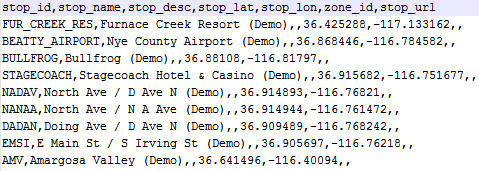
\includegraphics[width=8cm]{bspcsv.png}
	\caption{Hier sieht man wie so ein CSV-Format im Texteditor aussieht.}
	\label{fig:gtfs-dateiformat}
\end{figure}

Die verschiedenen Textfiles decken viele wichtige Informationen ab, die für ein GTFS benötigt werden.

\begin{tabular}{|l|c|l|}  \hline
	Dateiname & pflicht? & Definition \\ \hline
	agency.txt & ja & Geschäftsstellen die Daten zur Verfügung stellen \\ \hline
	stops.txt & ja & Haltestellen mit ihrer Position \\ \hline
	routes.txt & ja & Verkehrsverbindungen (Linien) mit den Fahrzeugarten \\ \hline %(zeitunabhängig)
	trips.txt & ja & Fahrten  \\ \hline												%(zeitabhängig)
	stop\_times.txt & ja & Zeiten in der Fahrzeuge Ankommen/Abfahren an Haltestellen \\ \hline
	calendar.txt & ja & Fahrplanveränderungen (Jahreszeiten) \\ \hline
	calendar\_dates & optional & Ausnahmeplan für bestimmtes Datum \\ \hline
	fare\_attributes.txt & optional & Fahrpreise und die Art der Bezahlung \\ \hline
	fare\_rules.txt & optional & Fahrpreisregeln verschiedener Zonen  \\ \hline
	shapes.txt & optional & Beschreibt den Weg eines Fahrzeuges (Darstellung) \\ \hline
	frequencies.txt & optional & Fahrpläne ohne fixe stop Zeiten. \\ \hline
	transfers.txt & optional & Umsteigpunkte verschiedener Routen (Linien) \\ \hline
	feed\_info.txt & optional & Zusätzliche Informationen über den Datensatz \\ \hline	
\end{tabular}
\cite{gtfsInhalt}
Daten die bisher nicht von der Plattform zur Verfügung gestellt werden: fare\_attributes.txt, fare\_rules.txt, frequencies.txt. 

\begin{figure}[]
	\centering
	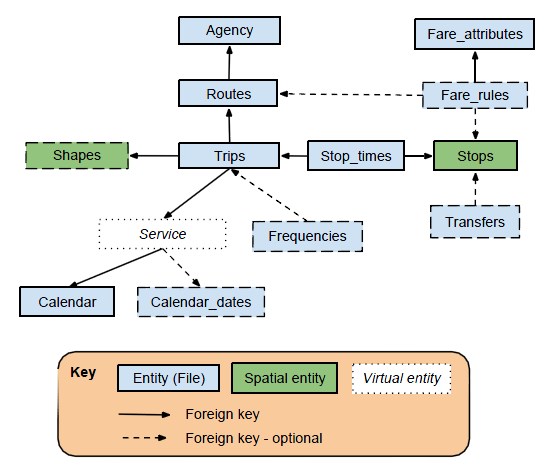
\includegraphics[scale=0.75]{GTFS_data_model_diagram.png}
 	\caption{Diese Übersicht zeigt die Abhängigkeiten der einzelnen Files.z.B. Braucht das Trips-File die Info der Route-Files(route\_id) um zu wissen auf welchem Weg diese Reise stattfindet.  \cite{gtfsUebersicht}}
	\label{fig:gtfs-uebersicht}
\end{figure}

 

\subsubsection{Vor- und Nachteile}
\label{sec:gtfs-vornachteile}
Die Daten können einfach von Mensch und Maschine gelesen werden, wegen dem einfachen Aufbau der Textfiles. Zudem stellt Google hierfür eine sehr gute Anleitung zur Verfügung, wie diese Daten verwendet werden und aufgebaut sind.

\subsection{GTFS Realtime (GTFS-RT)}
\label{sec:gtfs-rt}
GTFS-RT ist eine Erweiterung der GTFS-Static Daten. Wie der Name Realtime schon sagt handelt sich hier um Echtzeitdaten. 
\subsubsection{Datenstruktur}
\label{sec:gtfs-rt-datenstruktur}
GTFS-RT stellt folgende Daten zusätzlich in diesem Format zur Verfügung. Die Daten werden geschrieben/gelesen basierend auf sogenannten "Protocol Buffers", die stehen in vielen Programmiersprachen zur Verfügung (C++,C, Go, Java, Python).\cite{gtfs-rt}
\begin{itemize}
	\item{\textbf{Trip Updates}} -Hier werden Aktuelle Verspätungen, geänderte Routen, Ersatzfahrzeuge oder Ausfälle publiziert.  
	\item{\textbf{Service Alerts}} -Hier werden Informationen über Probleme mit Stationen,  Linien, das Ganze Netzwerk etc. übermittelt. 
	\item{\textbf{Vehicle Positions}} -Hier werden Daten geliefert die eine genaue Position des Vehicles mit der dazugehörigen Zeit liefert.\cite{gtfs-rt-google} 
\end{itemize}


\subsubsection{Vor- und Nachteile}
\label{sec:gtfs-rt-vornachteile}
Google stellt auch hier eine Gute Übersichtliche Anleitung zur Verwendung von GTFS-RT zur Verfügung.

\subsection{Fahrplan Hafas Rohdaten Format (HRDF)}
\label{subsec:hrdf}
Neben GTFS ist HRDF ein weiteres Dateiformat das die Fahrplandaten zur Verfügung stellt. 
Dieses Dateiformat kommt von der Firma HaCon. Das Format wird für ihren eigenen Journey Planner (HaCon Fahrplan-Auskunfts-System (HAFAS)) genutzt. Zudem stellt HaCon eine Plannungssoftware (Train Planning System TPS) für Infrastrukturbetreiber (wie Eisenbahnverkehrsunternehmen usw.) zur Verfügung. HRDF ist somit ihr eigenes Datenaustauschformat von Fahrplandaten.\cite{haconUebersicht}


\begin{figure}[]
	\centering
	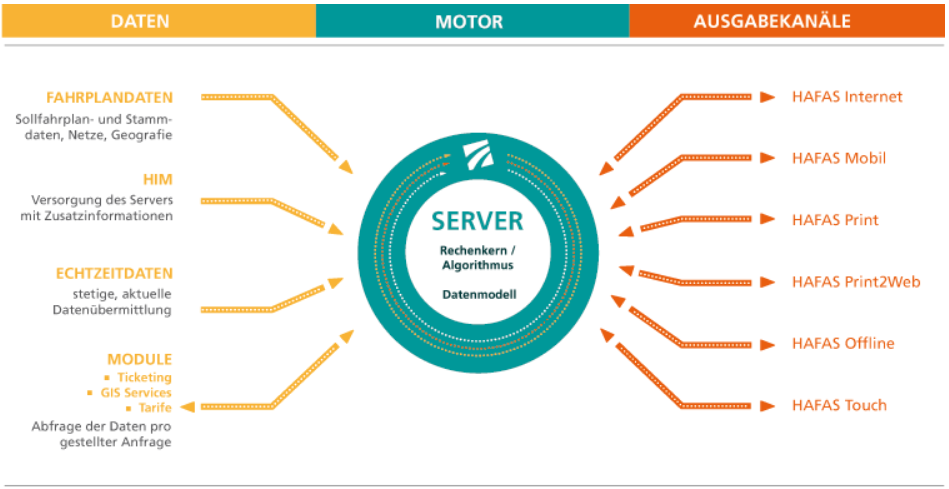
\includegraphics[width=12cm]{HAFAS.png}
	\caption{Dies ist eine Übersicht wie das HAFAS System aufgebaut ist. Die Fahrplandaten entsprechen hier dem HRDF-Format. \cite{haconUebersicht}}
	\label{fig:hafas-uebersicht}
\end{figure}



\subsubsection{Datenstruktur}
\label{sec:hrdf-datenstrukur}
Ähnlich wie GTFS-Files sind auch HRDF-Files auch Textfiles aber mit dem Unterschied das die Werte im Stil Tab-separated values (TSV) angelegt sind. Die Struktur der Daten ist etwas anders und um einiges komplizierter als bei GTFS. Auch sind die Daten oft schwerer zu lesen von Auge, weil sie manchmal als Bitfeld abgelegt sind. Nebenbei können HRDF Daten auch in GTFS-Daten konvertiert werden.\cite{hrdfintogtfs}
\begin{figure}[]
	\centering
	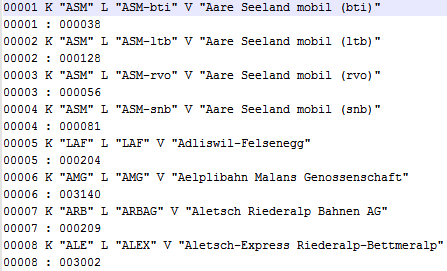
\includegraphics[width=8cm]{bsptsv.png}
	\caption{Hier sieht man wie so ein TSV-Format im Texteditor aussieht.}
	\label{fig:hrdf-dateiformat}
\end{figure}


\subsubsection{Vor- und Nachteile}	
\label{sec:hrdf-vornachteile}
Die Plattform warnt vor Verwendung der HRDF-Daten: "Die HRDF-Datei(en) sind relativ komplex. Ohne Not sollte nicht damit gearbeitet werden."\cite{opentransporthrdf}

\subsection{Fahrplan Überblick (timetable overview)}
\label{sec:Fahrplan Ueberblick}
Die Datei enthält alle Informationen der vorhandenen Fahrplandaten. Zusätzlich wird das Format(HRDF/GTFS) der Status, Gültigkeit und den Permalink der Fahrplandaten zur Verfügung gestellt.

\begin{figure}[]
	\centering
	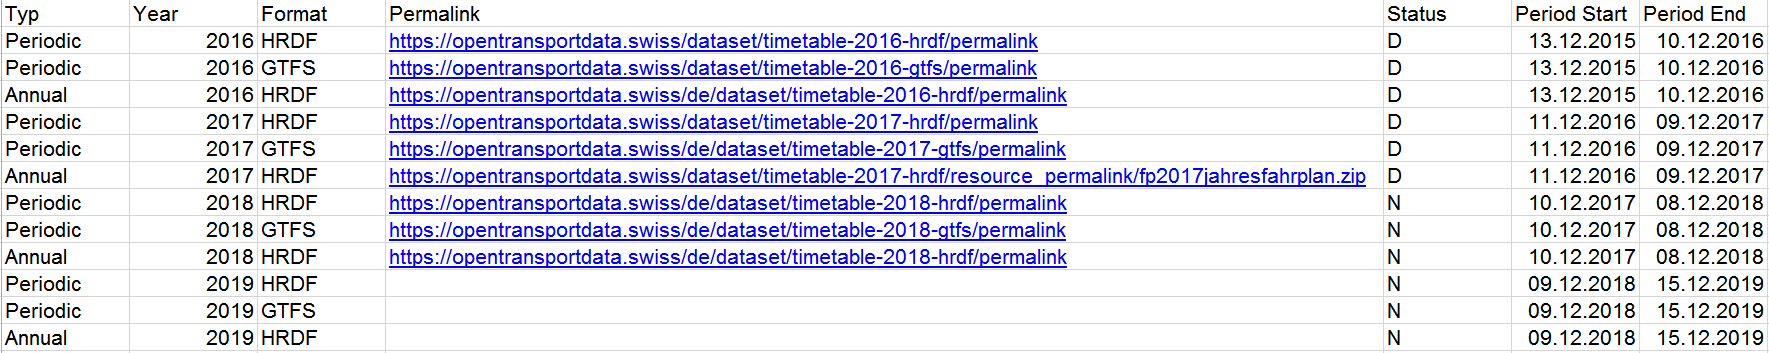
\includegraphics[width=12cm]{fahrplanueberblick.png}
	\caption{Die Fahrplan Überblick Datei wird hier in einer Excel Tabelle zur Verfügung gestellt.}
	\label{fig:Fahrplan Ueberblick dateiformat}
\end{figure}

\subsection{Ist-Daten (actual data)}
\label{sec:istdaten}
Bei den Ist-Daten handelt es sich um eine Ansammlung von Daten, welche die effektive gefahrenen Fahrten des letzten Tages enthalten. Somit sind diese Daten eigentlich in dem Sinne keine wirklichen Ist-Daten. Diese Daten können aber durchaus interessant sein für Statistiken:\cite{istdaten}
\begin{itemize}
	\item{Pünktlichkeit}   
	\item{Regelmässigkeit}. 
	\item{Anschlussqualität}  
\end{itemize}
Die Daten werden im CSV-Format bereitgestellt.

\subsection{Dienststellendokumentation (DiDok)}
\label{sec:didok}
Bei dieser Dokumentation geht es um die Daten zur Verwaltung der Stammdaten aller Dienststellen(Haltestellen) des öffentlichen Verkehrs der Schweiz. In dem Format werden Daten wie offizieller Name einer Haltestelle und die dazugehörige verantwortliche Geschäftsorganisation. Es werden aber auch die geographischen Koordinaten der Haltestellen mitgeliefert. Die Datei wird im Excel Format zur Verfügung gestellt.Die DiDok Daten werden vom BAV(Bundesamt für Verkehr) veröffentlicht. \cite{didok}

\begin{figure}[]
	\centering
	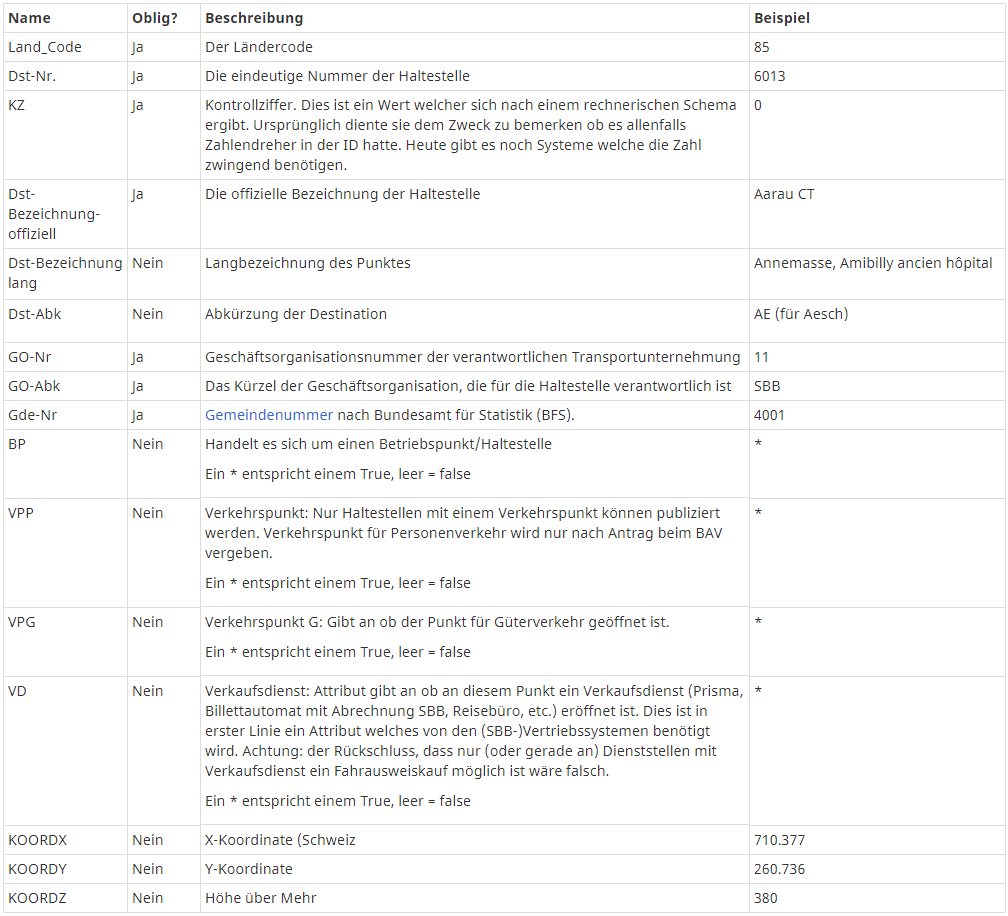
\includegraphics[width=15cm]{didokuebersicht.png}
	\caption{Hier sieht man ein Beispiel(Haltestelle) für das DiDok-File inklusive der Beschreibung einzelner Attribute.\cite{didok}}
	\label{fig:didok-uebersicht}
\end{figure}

\subsection{Geschäftsorganisationen (business organisations)}
\label{Geschaeftsorganisationen}
Die Daten werden im Excel-Format zur Verfügung gestellt. Hierbei findet man alle in der Schweiz operierenden Geschäftsorganisationen.
\begin{figure}[]
	\centering
	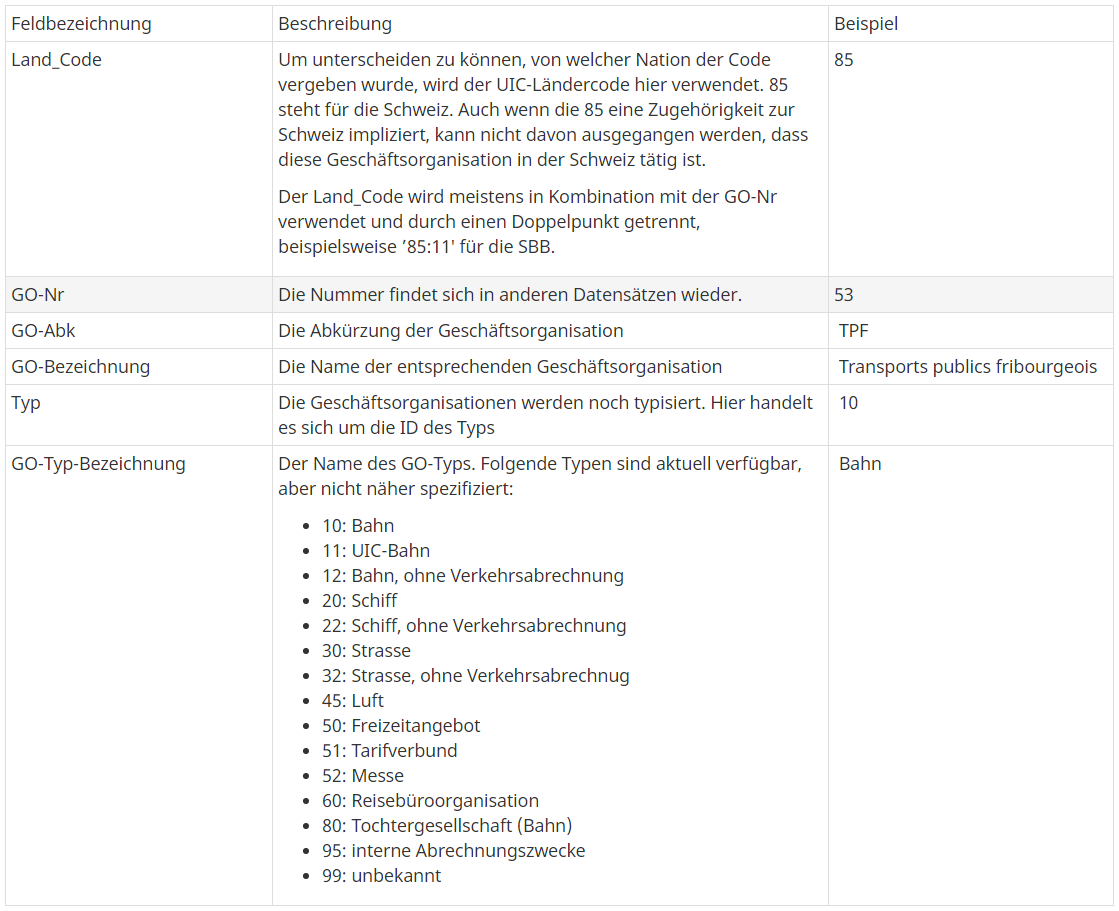
\includegraphics[width=12cm]{GOuebersicht.png}
	\caption{Beispiel einer Geschäftsorganisation mit Beschreibung der Attribute. \cite{geschaeftsorganisation}}
	\label{fig:Uebersicht Geschaeftsorganisationen}
\end{figure}
\subsubsection{Geschäftsorganisationen mit Echtzeit}
\label{Geschaeftsorganisationen mit Echtzeit}
Hierbei werden alle Geschäftsorganisationen erwähnt, die Echtzeitdaten liefern. Die Daten werden hier auch im Excel-Format zur Verfügung gestellt.

\begin{figure}[]
	\centering
	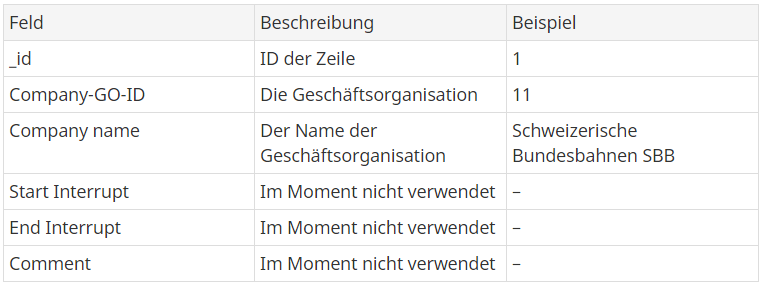
\includegraphics[width=12cm]{GO-Realtime.png}
	\caption{Beschreibung der Daten (Geschäftsorganisationen mit Echtzeit) anhand von einem Beispiel.\cite{geschaeftsorganisation-rt}}
	\label{fig:Uebersicht Geschaeftsorganisationen Echtzeit}
\end{figure}

\subsection{GA-HTA-Liste}
\label{GA-HTA-Liste}
In diesem Datensatz werden die Anzahl der General- (GA) und Halbtax-Abonnemente (HTA) pro Postleitzahl bereitgestellt mit dem dazugehörigen Erfassungsjahr. Diese Daten werden benötigt um Verkehrsmodelle zu verbessern, auf kantonaler und lokaler Basis.

\begin{figure}[]
	\centering
	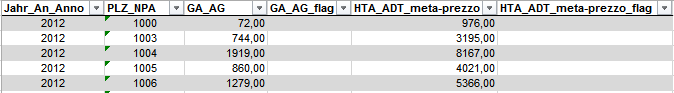
\includegraphics[width=12cm]{bspGA-HTA-Liste.png}
	\caption{Ausschnitt der Daten in einer GA-HTA-Liste  \cite{gahtaliste}}
	\label{fig:Beispiel GA-HTA-Liste}
\end{figure}
\begin{tabular}{|l|l|}  \hline
	Attribut & Beschreibung \\ \hline
	Jahr\_An\_Anno & Jahr des Stichdatums des Datenauszugs.  \\ \hline
	PLZ\_NPA & Vierstellige Postleitzahl gemäss Ortschaftenverzeichnis \\ \hline
	GA\_AG & Anzahl Generalabonnemente im Umlauf per Stichdatum. \\ \hline
	GA\_AG\_flag & Mittelwert Generalabonnemente, die weniger als 20Abos. \\ \hline
	HTA\_ADT\_meta-prezzo & Anzahl Halbtaxabonnemente im Umlauf per Stichdatum. \\ \hline	
	HTA\_ADT\_meta-prezzo\_flag & Mittelwert Halbtaxabonnemente, die weniger als 20Abos \\ \hline
\end{tabular}


\subsection{Bahnhofsliste (station list)}
\label{Bahnhofsliste}
Die Bahnhofsliste besteht aus zwei Dateien:
\begin{itemize}
	\item{\textbf{Station list}} - Hier sind alle Haltestellen der Schweiz enthalten, mit ID und Name.   
	\item{\textbf{Station geographic}} -Hier werden die Koordinaten für die Haltestellen zur Verfügung gestellt.
\end{itemize}
Die Dateien werden im CSV-Format bereitgestellt.
Die Station List entspricht die im HRDF-Format die "BAHNHOF"  Datei.\cite{bahnhofsliste}

\subsection{Abfahrts-/Ankunftsanzeiger (departure/arrival display)}%API
\label{sec:Abfahrts-/Ankunftsanzeiger}
Der Abfahrts- und Ankunftsanzeiger wird als Open Service API (application programming interface) zur Verfügung gestellt. Um die API zu benutzen muss man eine Haltestelle aus der Bahnhofsliste (station list) oder DiDok auswählen. Über diese API können mittels XML (Extensible Markup Language) Anfragen gestellt werden. Zusätzlich wird aber ein API-Key benötigt um Zugriff auf die API zu bekommen. Man verwendet sie für Haltestellenanzeiger. \cite{abfahrts-ankunftsanzeige}

\begin{figure}[]
	\centering
	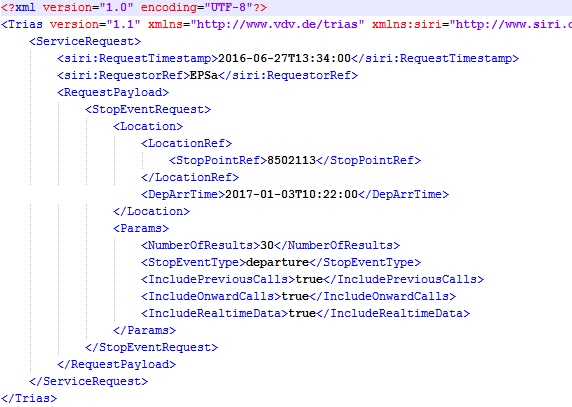
\includegraphics[width=12cm]{bspAbfrageAnkunftAbfahrt.png}
	\caption{Beispielcode einer Abfahrts-/Ankunft-Anfrage. Die Parameter, die Übergeben werden sind in schwarzer Schrift dargestellt.\cite{abfahrts-ankunftsanzeige}}
	\label{fig:Beispiel Anfrage Abfahrts-/Ankunftsanzeiger}
\end{figure}
\begin{tabular}{|l|l|}  \hline
	Parameter & Beschreibung \\ \hline
	8502113 & (StopPointRef) Haltestellencode Didok oder Bahnhofsliste   \\ \hline
	2017-01-03T10:22:00 & (DepArrTime)Ankunfts oder Abfahrtszeit \\ \hline
	30 & (NumberOfResults)Anzahl Resultate (maximal 40) \\ \hline
	departure & (StopEventType) entweder departure(Abfahrt) oder arrival(Ankunft) \\ \hline
	true & (IncludePreviousCalls)Haltestellen vor gesuchter Haltestelle mitliefern? \\ \hline	
	true & (IncludeOnwardCalls)Haltestellen nach gesuchter Haltestelle mitliefern? \\ \hline
	true & (IncludeRealtimeData)Sollen Echtzeitdaten mitgeliefert werden? \\ \hline
\end{tabular}

\subsection{Fahrtprognose (trip forecast)}%API
\label{sec:Fahrtprognose}
Wie auch beim Abfahrts- und Ankunftsanzeiger wird auch hier die Fahrprognose als Open Service API zur Verfügung gestellt.Ebnfalls wird auch hier über XML Anfragen gestellt und es wird auch ein API-Key benötigt.Sehr wichtig ist die JourneyRef(Fahrt-ID) diese muss bekannt sein und kann nicht über ein Sollfahrplan abgleitet werden, stattdessen wird sie über andere API-Request(TripRequest oder Ankunfts- und Abfahrtsanzeiger) abgeleitet.\cite{fahrtprognose}

\begin{figure}[]
	\centering
	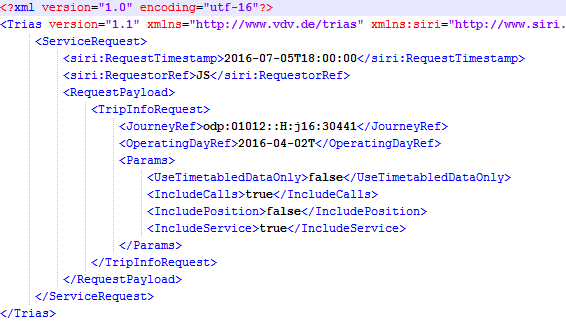
\includegraphics[width=12cm]{bspAbfrageFahrprognose.png}
	\caption{Beispielcode einer Fahrtprognose-Anfrage. Die Parameter, die Übergeben werden sind in schwarzer Schrift dargestellt.\cite{fahrtprognose}}
	\label{fig:Beispiel Anfrage Fahrtprognose}
\end{figure}

\begin{tabular}{|l|l|}  \hline
	Parameter & Beschreibung \\ \hline
	odp:01012::H:j16:30441& (JourneyRef)wird über andere Quellen bezogen/hergestellt   \\ \hline
	2016-04-02T & (OperatingDayRef)Betriebstag \\ \hline
	false & (UseTimetabledDataOnly)Infos zu Verkehrstagen ausgegeben werden? \\ \hline
	true & (IncludeCalls)Sollen Halte der Fahrt ausgegeben werden?   \\ \hline
	false & (IncludePosition)Aktuelle Position des Fahrzeugs mitliefern? \\ \hline	
	true & (IncludeService)Verkehrsmittelinformationen ausgeben? \\ \hline
\end{tabular}
	
	\section[Algorithmen]{Algorithmen}
\label{sec:Algorithmen}
Die für einen Jouney Planner zu lösende Aufgabe ist das Shortest-Path Problem. Un dieses Problem zu lösen, gibt es mehrere Herangehensweisen. 

\subsection{Graph Basierte Algorithmen}
\label{sec:Graph Basierte Algorithmen}
Graph-Basierte Algorithmen bilden einen Graphen aus Punkten. Die Verbindungen zwischen den Punkten werden mit einer Gewichtung versehen. Der Algorithmus iteriert nun über den Graphen und findet die Verbindung zwischen dem Start- und Endpunkt mit dem niedrigsten kombinierten Gewicht.

\subsubsection{Dijkstra}
\label{sec:Dijkstra}
Der Dijkstra Algorithmus ist ein Single-Source-Shortest-Path Algorithmus. Er berechnet den kürzesten Weg von einem Startnode zu jedem anderen \gls{Node} im Graphen. Er iteriert über alle möglichen Verbindungen und speichert das Gewicht eines Zielnodes. Wenn eine weitere Verbindung zum gleichen Node gefunden wird, so wird die Verbindung mit dem geringsten Gewicht behalten. Es wird immer die Node mit dem geringsten Gewichtswert zum Startnode als nächstes berechnet. Wenn auch der Zielnode bekannt ist, wird der Algorithmus gleichzeitig vom Start und Zielnode aus gestartet, so dass sie sich in der Mitte treffen. 

Der Dijkstra Algorithmus ist der Basisalgorithmus mit dem die anderen Algorithmen verglichen werden. Er ist konzeptionell einfach, jedoch in keiner Weise optimiert. Die Laufzeit erhöht sich exponentiell mit der Anzahl der Nodes und Verbindungen, weshalb er für grosse Netzwerke ungeeignet ist. ~\cite{dij_a} ~\cite{dij_bell}

\subsubsection{A*}
\label{sec:A*}
Der A* Algorithmus ist eine Erweiterung des Dijkstar Algorithmus. Er sucht nicht wie der Dijkstra Algorithmus linear in alle Richtungen, sondern gezielt in Richtung des Zielnodes. Dazu wird jedem Punkt im Graph eine Entfernung zum Zielnodes zugewiesen. Nun wird dieser Wert mit dem Gewichtswert des Abstandes zum Startnode kombiniert. Der als nächstes zu berechnende Punkt wird nun aufgrund dieses Wertes entschieden. Dadurch werden Verbindungen welche in Richtung des Zieles führen präferiert und es werden viele überflüssige Rechenschritte eingespart.

Obwohl der A* Algorithmus mehr Operationen pro Node durchführen muss, hat er dennoch eine höhere Performance als der Dijkstra Algorithmus, da viel weniger Nodes untersucht werden müssen. Der Nachteil vom A* Algorithmus ist, dass er mehr Memory benötigt. ~\cite{dij_a}

 

\subsubsection{Bellman-Ford}
\label{sec:Bellman-Ford}
Der Bellman-Ford Algorithmus verwendet das gleiche Grundkonzept wie der Dijkstra Algorithmus. Er achtet jedoch nicht auf den geringsten Gewichtungsfaktor zum Startnode, sondern geht der Reihe nach alle Nodes durch. Wenn nun für einen Node nicht alle Zwischennodes zum Starnode schon berechnet wurden, so scheint dieser Node unerreichbar. Um diese Problematik zu lösen wird dieser Prozess x-1 mal wiederholt, wobei x die Anzahl der Nodes ist. ~\cite{dij_bell} ~\cite{bell}

Der Bellman-Ford Algorithmus ist langsamer als der Dijkstra Algorithmus, da er mehrere Durchläufe über alle Nodes benötigt. Dies bietet ihm jedoch den Vorteil, dass auch eine negative Gewichtung einer Verbindung möglich ist.

\subsection{Non Graph Basierte Algorithmen}
\label{sec:Non Graph Basierte Algorithmen}
In diesem Abschnitt werden Algorithmen erläutert, welche nicht auf das Grundkonzept des Dijkstra Algorithmus aufbauen.

\subsubsection{RAPTOR}
\label{sec:RAPTOR}
Der Round-Based Public Transit Routing Algorithmus, auch RAPTOR Algorithmus genannt, ist ein Rundenbasierter, auf öffentliche Verkehrsnetzwerke zugeschnittener Algorithmus, welcher auf die vorgegebenen Zuglinien achtet.

Der RAPTOR Algorithmus durchläuft mehrere Runden um von der Startstation zur Zielstation zu finden. In der ersten Runde werden alle Zuglinien gescannt, welche durch die Startstation verlaufen. Wenn eine andere Zuglinie die gescannte Zuglinie kreuzt, so wird die andere Zuglinie sowie die Kreuzungsstation markiert. In der nächsten Runde werden nun alle markierten Zuglinien gescannt. Dieser Prozess wird so lange weitergeführt, bis sich die Zielstation in einer gescannten Zuglinie befindet. Nun kann anhand der Kreuzungsstationen die Route erstellt werden.

Der RAPTOR Algorithmus besitzt eine höhere Performanz als alle Graph Basierten Algorithmen. ~\cite{raptor}

\subsubsection{Connection Scan Algorithm}
\label{sec:Connection Scan Algorithm}
Der Connection Scan Algorithm, kurz CSA, ist schon vom Grundkonzept her auf Zeitplanbasierte Netzwerke zugeschnitten. Er arbeitet mit Stations\gls{stations}, Connections\gls{connections}, Trips\gls{trips} und Footpaths\gls{footpaths}. 

In einem Ersten Schritt werden die Daten in die benötigte Timetable-Form gebracht und alle Connections nach der Abfahrtszeit sortiert. Diese Schritte werden preprocessed. Danach wird über alle Connections iteriert. Eine Connection wird als erreichbar markiert, wenn sie an bereits als erreichbar markierte Connections anschliesst oder mit der Startstation verbunden ist. Dies wird dann solange durchgeführt, bis die Zielstation erreicht ist. Anschliessend wird von der Zielstation aus der verfolgte Weg zusammengesetzt, so dass ein Journey von der Startstation zur Zielstation entsteht. 

Für grosse Netzwerke kann der CSA mit einem Quadtree-Preprocessing Schritt erweitert werden. Dabei wird das Netzwerk in immer kleiner werdende Quadrate unterteilt. Für Quadrate welche nicht die Start- oder Zielstation enthalten, müssen nun nur noch die Connections beachtet werden, welche über die Ränder des Quadrates hinaus gehen. Somit können für Fernverbindungen die lokalen Connections ignoriert werden.
\begin{figure}[]
	\centering
	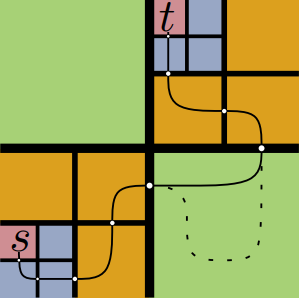
\includegraphics[width=8cm]{QuadTree.png}
	\caption{Veranschaulichung der Funktion des QuadTree-Preprocessings ~\cite{csa}}
	\label{fig:QuadTree}
\end{figure}


Im Gegensatz zum Dijkstra müssen beim CSA die Connections nicht nach dem nächsten Schritt durchsucht werden, da die Abfolge durch die Preprocessing-Schritte schon definiert wurde. Dies führt zu einer Performanceverbesserung im mehrstelligen Bereich. Ein Nachteil ist jedoch, dass Preprocessing-Schritte von Nöten sind und so nicht in echtzeit auf Verspätungen reagiert werden kann. Da diese Schritte jedoch nur wenige Sekunden benötigen ist dies kein schwerwiegender Nachteil. Mit der Erweiterung des Quadtree-Preprocessings können auch Anfragen in landesweite Netzwerke in wenigen Millisekunden berechnet werden. 

Im Vergleich zum RAPTOR Algorithmus bietet der CSA eine höhere Performance. ~\cite{csa}


\subsection{Transfer Pattern}
\label{sec:Transfer Pattern}
Transfer Pattern ist eine Algorithmusstrategie welche auf Preprocessing setzt. Alle möglichen Verbindungen werden mithilfe eines Algorithmuses berechnet und in einem Datensatz gespeichert. Die eigentliche Anfrage beschränkt sich dann auf eine Query-Abfrage auf diesen Datensatz.

Für das Preprocessing können alle zuvor genannten Algorithmen verwendet werden. Die Dijksta basierten Algorithen haben jedoch den Nachteil, dass Query anfragen für landesweite Netzwerke immer noch mehrere Sekunden benötigen, weshalb der RAPTOR Algorithmus oder der CSA zu bevorzugen sind. ~\cite{transferpatterns_alenex}

Um das Preprocessing zu beschleunigen können mehrere Erweiterungen hinzugefügt werden. Eine davon ist die Verwendung von Hubs. Dabei werden die grössten Stationen als Hubs markiert. Zwischen diesen Hubs werden alle Transfer Pattern berechnet. Bei Stationen welche keine Hubs sind werden nur die Verbindungen bis zum nächsten Hub berechnet. Sollte nach drei Zugwechseln kein Hub erreicht sein so wird die Verbindung verworfen. Dies kann zwar zu Fehlern führen, ist aber vernachlässigbar, da die Fehlerrate laut Experimenten bei drei Promille liegt. ~\cite{transferpatterns_esa}

Der Preprocessing\gls{preprocessing} kann je nach Grösse und Struktur des Netzwerks eine lange Zeit in Anspruch nehmen. Selbst mit allen Erweiterungen braucht das Preprocessing für das CH-Netzwerk vier Stunden. Dafür benötigen die Query-Anfragen nur wenige Millisekunden. Der Nachteil ist jedoch, dass mit Transfer Pattern nicht auf Zugverspätungen und Fahrplanänderungen reagiert werden kann. 






	
	

\section[Programme]{Programme}
\label{sec:programme}

Es gibt viele Journey-Planning-Softwares, doch nur wenige davon besitzen eine OpenSource-Lizensierung. Wir werden uns im Rahmen dieses Projektes auf die OpenSource Anwendungen beschränke.

\subsection{Traintickets.to} 
\label{sec:Traintickets.to}

Traintickets.to ist ein von Linus Norton ~\cite{LinusNorton} entwickelter Journey Planner für das englische Zugnetzwerk. Linus Norton ist CTO der Firma Assertis ~\cite{assertis}, welche das Projekt betreibt. ~\cite{noauthor_so_nodate}


Traintickets.to basiert auf einem modifizierten CSA kombiniert mit TransferPattern. In einem preprocessing Schritt werden aus einem modifizierten GTFS-datasheet die TransferPattern mit dem CSA generiert. Diese werden dann von Hauptprogramm gefiltert und über eine API zur Verfügung gestellt. Assertis ist von der ATOC (Association of Train Operation Companies) lizensiert, so dass sie Ticketpreise anzeigen können sowie Tickets direkt verkaufen können.

Traintickets.to besitzt zwei verschiedene Lizensierungen. Die TransferPattern generierung sowie das Filterprogramm stehen unter einer GNU GPLv3 Lizenz. Die WebAPI ist technisch gesehen ein eigenes Projekt und steht unter exclusive copyright.

Vorteil der Traintickets.to Anwendung ist, dass dieser schon Landesweit implementiert und getestet ist und deshalb auf der Schweiz ohne Skalierung anwendbar ist. ~\cite{testus} ~\cite{noauthor_train_nodate}

Nachteile der Traintickets.to Anwendung sind, dass modifizierte GTFS-Daten verwendet werden und diese so nicht direkt von der OpenData platform bezogen werden können, dass der Code schlecht Strukturiert ist und dass die Anwendung aufgrund des preprocessing-Aufbaus nicht auf Verspätungen und Fahrplanänderungen reagieren kann.
     


\subsection{Open Trip Planner}
\label{sec:OTP}

Der OpenTripPlanner kurz OTP ist eine auf der Maven-Repository aufbauende Multimodale trip planning Software welche anfangs für Städte ausgelegt war, nun aber auch in ersten landesweiten Netzwerken Anwendung findet. Er wurde von einem OpenSource-Kollektiv aus mehr als 100 Personen in acht Jahren entwickelt. 

Der OTP basiert auf dem A*-Algorithmus und verwendet GTFS-Daten und OpenStreetMap Daten in Form einer pbf-Datei. In einem preprocessing Schritt wird der Graph für den Algorithmus erstellt. Dieser kann in einer Datei gespeichert werden oder direkt im RAM des Servers gelagert werden. Selbiges wird für die OpenStreetMap-Daten gemacht. Während dem Betrieb kann der Graph angepasst werden, so dass das Programm auf verspätete Züge reagieren kann. 

OTP steht unter einer GNU Lesser General Public License. 

Vorteile des OTP sind, dass er in Echtzeit auf Fahrplanänderungen und Verspätungen reagieren kann, dass OTP schon seit mehreren Jahren in verschiedenen Städten implementiert und getestet ist und dass unsere Arbeit vom OpenSource-Kollektiv in den Hauptcode aufgenommen werden könnte. 

Nachteile des OTP sind, dass landesweite Implementationen erst in der Beta-Phase sind und somit noch nicht ausreichen getestet sind und dass das Programm unheimlich gross und verzweigt ist, so dass eine lange Einarbeitungszeit von Nöten ist.



\subsection{R5}
\label{sec:R5}

Rapid Realistic Routing on Real-world and Reimagined networks oder kurz R5 ist ein multimodales Trip-Planning-Tool. Er wurde von der Firma Conveyal entwickelt und basiert auf dem OTP. 

R5 hat die Grundstruktur des OTP übernommen, jedoch verwendet R5 den RAPTOR-Algorithmus anstelle des A*-Algorithmus. Dadurch wurden einige Programmstrukturen verändert, da der RAPTOR-Algorithm nicht auf den Dijkstra-Algorithmus aufbaut und auch keinen Graphen verwendet. 

R5 steht unter der MIT License. 

Vorteile des R5 sind, dass er in Echtzeit auf Fahrplanänderung und Verspätungen reagieren kann und dass der RAPTOR-Algorithmus eine bessere Performance als die Dijkstra-basierten Algorithmen bietet. 

Nachteile des R5 sind, dass er unter einer MIT License steht und dass der R5 von einer Firma entwickelt wurde, welche unsere Arbeit nicht übernehmen werden.
	
	\section[Erkenntnisse]{Erkenntnisse}
\label{sec:erkenntnisse}

\subsection{Daten}
\label{sec:erkenntnisseDaten}
Für unsere Anwendung ist der GTFS Datentyp dem HRDF Datentyp aus mehreren Gründen überlegen.
\begin{enumerate}
	\item Alle zuvor genannten Programme basieren auf dem GTFS-Datentyp. Dies führt
\end{enumerate}



\subsection{Algorithmen}
\label{sec:erkenntnisseAlgorithmen}



\subsection{Programme}
\label{sec:erkenntnisseProgramme}
Die drei Programme Traintickets.to, OTP und R5 wurden in Betracht gezogen. 

R5 basiert zwar auf dem modernen RAPTOR Algorithmus, ist jedoch nicht für unser Projekt geeignet. Der Programmcode steht unter einer MIT-Lizenz. R5 wird von der Firma Conveyal entwickelt. Wenn wir mit unserem Projekt auf das R5 Programm aufbauen, so besteht keine Chance dass unser Code in das Originalprogramm integriert wird.

Die beiden Programme "Traintickets.to" und "OpenTripPlanner" wurden genauer betrachtet. Die Programmierer beider Programme wurden von uns angeschrieben. Wir posteten eine Anfrage in die OTP Developer Mailing. Darin fragten wir ob sie zurzeit an einer implementation des CSA in ihrem Programm arbeiten und wie sie zu der Idee unseres Projektes stehen. Nach nur kurzer Zeit bekahmen wir eine Antwort. Eine integration des CSA ist zurzeit nicht geplant. Projekte von neuen Personen sind gerne gesehen, jedoch wird der Code nur in das Hauptprogramm übernommen, wenn  das OpenSource-Gremium den Code als gut erachtet. Dazu muss der Code den Programmrichtlinen entsprechen und der Strategie des OTP entsprechen. Die strategie des OTP liegt darin, dass sie nicht ausschliesslich auf die schnellste Lösung setzen. Wichtiger ist, dass das Programm in Echtzeit auf Verspätungen und Fahrplanänderungen reagieren kann. Wir haben auch Linus Norton von "Traintickets.to" angeschrieben, konnten jedoch keine Antwort erhalten.
	
	\section[AufgabeBA]{AufgabeBA}
\label{AufgabeBA}


\subsection{AufgabenstellungBA}
\label{AufgabenstellungBA}
\begin{itemize}
	\item Schreiben sie eine Implementation des CSA für den OpenTripPlanner. Dieser muss OTP-Development-Richtklinien konform sein.
	\item Implementieren sie die Schweizer GTFS und OpenStreetMap daten für den OTP, so dass Punkt zu Punkt Verbindungen in der Schweiz berechnet werden können.
	\item Implementieren sie den Schweizer realtime GTFS-Feed, so dass das Programm auf Verspätungen oder Fahrplanänderungen reagieren kann.
	\item Implementieren sie Skalierungsoptimierungen für das Programm, so dass es mit einem landesweiten System bessere Performanz liefert.
	\item Führen sie Performance Tests durch und vergleichen sie das Implementierte System mit dem auf Dijkstra basierenden OTP.
	\item Dokumentieren sie ihre Ergebnisse und schreiben sie einen ausführlichen Bericht.
\end{itemize}

\subsection{Lastenheft}
\label{Lastenheft}
\begin{tabular}{ | p{5cm} | l | l | }
	\hline
	\multicolumn{3}{|c|}{Funktionale Anforderungen} \\
	\hline
	Anforderung & Anforderungsart & Priorisierung \\
	\hline
	Der CSA muss als Berechnungsalgorithmus verwendet werden. & Muss & 1 \\
	\hline
	Es kann eine Verbindung zwischen 2 Stationen zu einem bestimmten Zeitpunkt errechnet werden. & Muss & 2 \\
	\hline
	Fusswege zu Stationen hin können miteinbezogen werden können. & Muss & 3 \\
	\hline
	Das Programm kann auf Verspätungen und Fahrplanänderungen reagieren. & Muss & 4 \\
	\hline
	Mehrere mögliche Verbindungen können angezeigt werden. & Muss & 5 \\
	\hline
	Fusswege zwischen verschiedenen Stationen können miteinbezogen werden. & Soll & 6 \\
	\hline
	Die Angezeigte Route soll den Fahrlinien, z.B. Schienen, folgen. & Kann & 7 \\
	\hline
\end{tabular}
\newline
\newline
\newline
Nicht funktionale Anforderungen
\begin{itemize}
	\item Der Programmcode muss den OTP-Development-Richtlinien entsprechen.
	\item Die Query-Zeit muss weniger als 1 Sekunde betragen.
	\item Die Preprocessing-Zeit muss weniger als 30 Minuten betragen.
	\item Die Query-Zeit soll schneller als die des originalen OTP sein.
\end{itemize}

\subsection{Meilensteine}
\label{Meilensteine}
\begin{enumerate}
	\item OTP Analysiert
	\item OTP mit dem Schweitzer System implementieren
	\item Basis CSA implementiert
	\item CSA Spalierungsoptimierung implementiert
	\item Performancetests durchgeführt
	\item Bericht geschrieben
\end{enumerate}

\subsection{Zeitplan}
\label{Zeitplan}
Der Zeitplan ist im beigelegten Excel-File ersichtlich.
	
	\newpage
	\listoffigures
		\bibliography{test2,Programme}
	\bibliographystyle{IEEEtran}
	

	
	
	
	
	
\end{document}